\documentclass{standalone}
\usepackage{tikz}
\usetikzlibrary{patterns, positioning}


\begin{document}
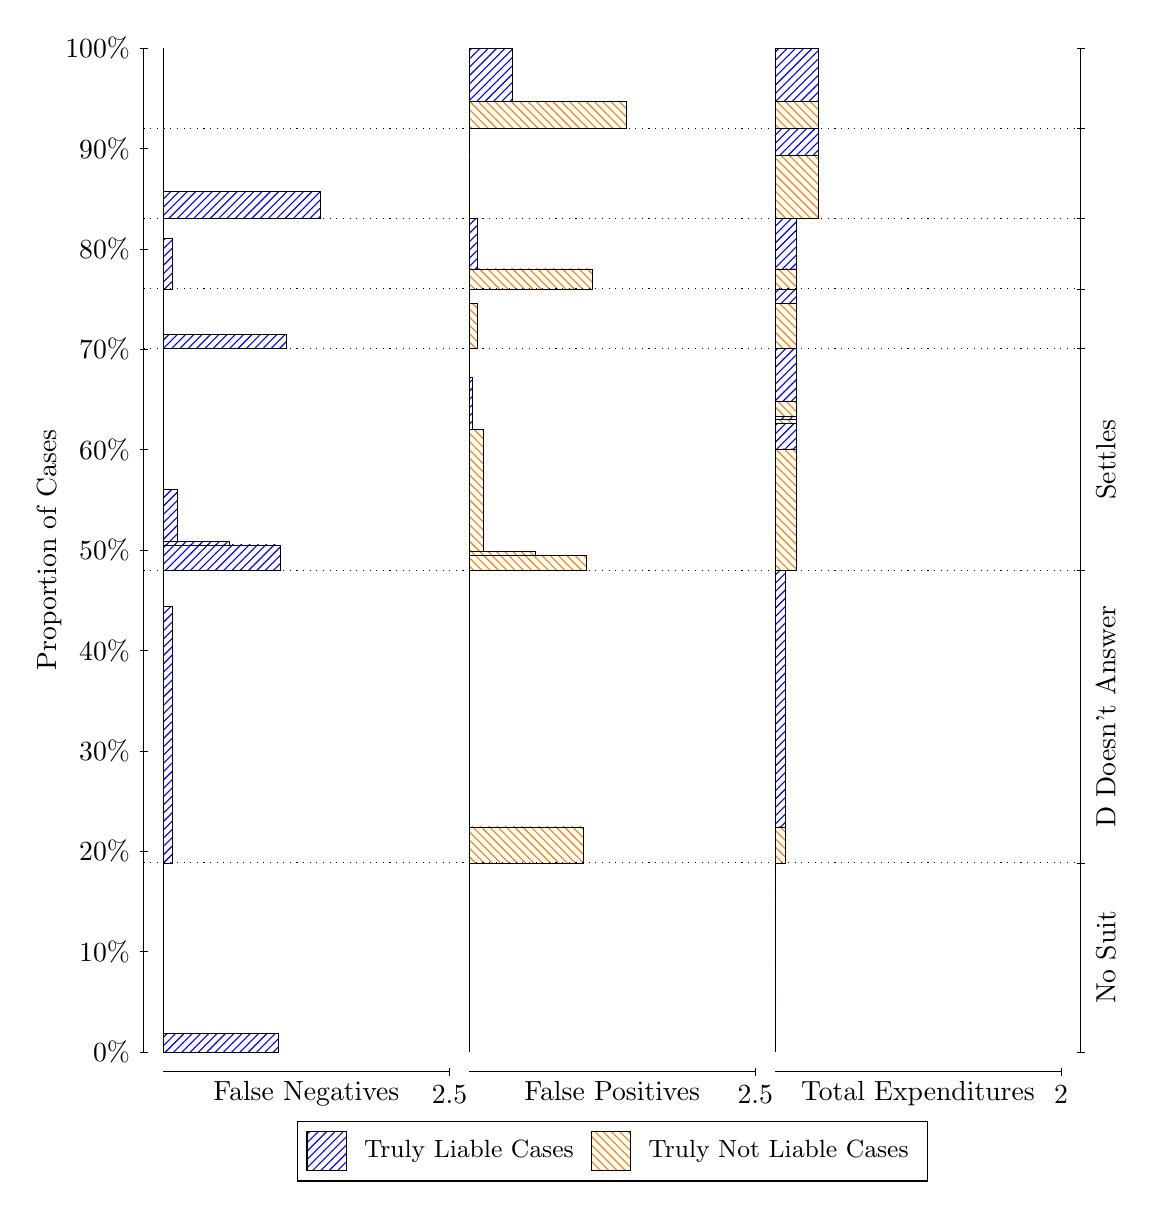
\begin{tikzpicture}
\draw[black, very thin] (1.5,1.75) -- (1.5,14.5);
\node[rotate=90, text=black, anchor=center] at (0.3, 8.125) {Proportion of Cases};
\draw[black, very thin] (1.45,1.75) -- (1.55,1.75);
\node[text=black, anchor=east] at (1.45, 1.75) {0\%};
\draw[black, very thin] (1.45,3.025) -- (1.55,3.025);
\node[text=black, anchor=east] at (1.45, 3.025) {10\%};
\draw[black, very thin] (1.45,4.3) -- (1.55,4.3);
\node[text=black, anchor=east] at (1.45, 4.3) {20\%};
\draw[black, very thin] (1.45,5.575) -- (1.55,5.575);
\node[text=black, anchor=east] at (1.45, 5.575) {30\%};
\draw[black, very thin] (1.45,6.85) -- (1.55,6.85);
\node[text=black, anchor=east] at (1.45, 6.85) {40\%};
\draw[black, very thin] (1.45,8.125) -- (1.55,8.125);
\node[text=black, anchor=east] at (1.45, 8.125) {50\%};
\draw[black, very thin] (1.45,9.4) -- (1.55,9.4);
\node[text=black, anchor=east] at (1.45, 9.4) {60\%};
\draw[black, very thin] (1.45,10.675) -- (1.55,10.675);
\node[text=black, anchor=east] at (1.45, 10.675) {70\%};
\draw[black, very thin] (1.45,11.95) -- (1.55,11.95);
\node[text=black, anchor=east] at (1.45, 11.95) {80\%};
\draw[black, very thin] (1.45,13.225) -- (1.55,13.225);
\node[text=black, anchor=east] at (1.45, 13.225) {90\%};
\draw[black, very thin] (1.45,14.5) -- (1.55,14.5);
\node[text=black, anchor=east] at (1.45, 14.5) {100\%};

\draw[black, very thin] (13.4,1.75) -- (13.4,14.5);
\draw[black, very thin] (13.35,1.75) -- (13.45,1.75);
\node[anchor=west] at (13.35, 1.75) {};
\draw[black, very thin] (13.35,4.1507) -- (13.45,4.1507);
\node[anchor=west] at (13.35, 4.1507) {};
\draw[black, very thin] (13.35,7.8663) -- (13.45,7.8663);
\node[anchor=west] at (13.35, 7.8663) {};
\draw[black, very thin] (13.35,10.682) -- (13.45,10.682);
\node[anchor=west] at (13.35, 10.682) {};
\draw[black, very thin] (13.35,11.441) -- (13.45,11.441);
\node[anchor=west] at (13.35, 11.441) {};
\draw[black, very thin] (13.35,12.338) -- (13.45,12.338);
\node[anchor=west] at (13.35, 12.338) {};
\draw[black, very thin] (13.35,13.48) -- (13.45,13.48);
\node[anchor=west] at (13.35, 13.48) {};
\draw[black, very thin] (13.35,14.5) -- (13.45,14.5);
\node[anchor=west] at (13.35, 14.5) {};

\draw[black, very thin, pattern color=blue, pattern=north east lines] (1.75,1.75) rectangle (3.2033,1.991);
\draw[black, very thin, pattern color=orange, pattern=north west lines] (1.75,1.991) rectangle (1.75,4.1507);
\draw[black, very thin, pattern color=blue, pattern=north east lines] (1.75,4.1507) rectangle (1.859,7.4086);
\draw[black, very thin, pattern color=orange, pattern=north west lines] (1.75,7.4086) rectangle (1.75,7.8663);
\draw[black, very thin, pattern color=blue, pattern=north east lines] (1.75,7.8663) rectangle (3.2397,8.1892);
\draw[black, very thin, pattern color=blue, pattern=north east lines] (1.75,8.1892) rectangle (2.5857,8.2304);
\draw[black, very thin, pattern color=blue, pattern=north east lines] (1.75,8.2304) rectangle (1.9317,8.8954);
\draw[black, very thin, pattern color=orange, pattern=north west lines] (1.75,8.8954) rectangle (1.75,10.682);
\draw[black, very thin, pattern color=blue, pattern=north east lines] (1.75,10.682) rectangle (3.3123,10.867);
\draw[black, very thin, pattern color=orange, pattern=north west lines] (1.75,10.867) rectangle (1.75,11.441);
\draw[black, very thin, pattern color=blue, pattern=north east lines] (1.75,11.441) rectangle (1.859,12.084);
\draw[black, very thin, pattern color=orange, pattern=north west lines] (1.75,12.084) rectangle (1.75,12.338);
\draw[black, very thin, pattern color=blue, pattern=north east lines] (1.75,12.338) rectangle (3.7483,12.684);
\draw[black, very thin, pattern color=orange, pattern=north west lines] (1.75,12.684) rectangle (1.75,13.48);
\draw[black, very thin, pattern color=orange, pattern=north west lines] (1.75,13.48) rectangle (1.75,13.827);
\draw[black, very thin, pattern color=blue, pattern=north east lines] (1.75,13.827) rectangle (1.75,14.5);
\draw[black, very thin, pattern color=orange, pattern=north west lines] (5.6333,1.75) rectangle (5.6333,3.9097);
\draw[black, very thin, pattern color=blue, pattern=north east lines] (5.6333,3.9097) rectangle (5.6333,4.1507);
\draw[black, very thin, pattern color=orange, pattern=north west lines] (5.6333,4.1507) rectangle (7.0867,4.6084);
\draw[black, very thin, pattern color=blue, pattern=north east lines] (5.6333,4.6084) rectangle (5.6333,7.8663);
\draw[black, very thin, pattern color=orange, pattern=north west lines] (5.6333,7.8663) rectangle (7.123,8.0595);
\draw[black, very thin, pattern color=orange, pattern=north west lines] (5.6333,8.0595) rectangle (6.469,8.1107);
\draw[black, very thin, pattern color=orange, pattern=north west lines] (5.6333,8.1107) rectangle (5.815,9.6531);
\draw[black, very thin, pattern color=blue, pattern=north east lines] (5.6333,9.6531) rectangle (5.6697,10.318);
\draw[black, very thin, pattern color=blue, pattern=north east lines] (5.6333,10.318) rectangle (5.6333,10.682);
\draw[black, very thin, pattern color=orange, pattern=north west lines] (5.6333,10.682) rectangle (5.7423,11.256);
\draw[black, very thin, pattern color=blue, pattern=north east lines] (5.6333,11.256) rectangle (5.6333,11.441);
\draw[black, very thin, pattern color=orange, pattern=north west lines] (5.6333,11.441) rectangle (7.1957,11.695);
\draw[black, very thin, pattern color=blue, pattern=north east lines] (5.6333,11.695) rectangle (5.7423,12.338);
\draw[black, very thin, pattern color=orange, pattern=north west lines] (5.6333,12.338) rectangle (5.6333,13.134);
\draw[black, very thin, pattern color=blue, pattern=north east lines] (5.6333,13.134) rectangle (5.6333,13.48);
\draw[black, very thin, pattern color=orange, pattern=north west lines] (5.6333,13.48) rectangle (7.6317,13.827);
\draw[black, very thin, pattern color=blue, pattern=north east lines] (5.6333,13.827) rectangle (6.1783,14.5);
\draw[black, very thin, pattern color=orange, pattern=north west lines] (9.5167,1.75) rectangle (9.5167,3.9097);
\draw[black, very thin, pattern color=blue, pattern=north east lines] (9.5167,3.9097) rectangle (9.5167,4.1507);
\draw[black, very thin, pattern color=orange, pattern=north west lines] (9.5167,4.1507) rectangle (9.6529,4.6084);
\draw[black, very thin, pattern color=blue, pattern=north east lines] (9.5167,4.6084) rectangle (9.6529,7.8663);
\draw[black, very thin, pattern color=orange, pattern=north west lines] (9.5167,7.8663) rectangle (9.7892,9.4087);
\draw[black, very thin, pattern color=blue, pattern=north east lines] (9.5167,9.4087) rectangle (9.7892,9.7316);
\draw[black, very thin, pattern color=orange, pattern=north west lines] (9.5167,9.7316) rectangle (9.7892,9.7828);
\draw[black, very thin, pattern color=blue, pattern=north east lines] (9.5167,9.7828) rectangle (9.7892,9.8239);
\draw[black, very thin, pattern color=orange, pattern=north west lines] (9.5167,9.8239) rectangle (9.7892,10.017);
\draw[black, very thin, pattern color=blue, pattern=north east lines] (9.5167,10.017) rectangle (9.7892,10.682);
\draw[black, very thin, pattern color=orange, pattern=north west lines] (9.5167,10.682) rectangle (9.7892,11.256);
\draw[black, very thin, pattern color=blue, pattern=north east lines] (9.5167,11.256) rectangle (9.7892,11.441);
\draw[black, very thin, pattern color=orange, pattern=north west lines] (9.5167,11.441) rectangle (9.7892,11.695);
\draw[black, very thin, pattern color=blue, pattern=north east lines] (9.5167,11.695) rectangle (9.7892,12.338);
\draw[black, very thin, pattern color=orange, pattern=north west lines] (9.5167,12.338) rectangle (10.062,13.134);
\draw[black, very thin, pattern color=blue, pattern=north east lines] (9.5167,13.134) rectangle (10.062,13.48);
\draw[black, very thin, pattern color=orange, pattern=north west lines] (9.5167,13.48) rectangle (10.062,13.827);
\draw[black, very thin, pattern color=blue, pattern=north east lines] (9.5167,13.827) rectangle (10.062,14.5);
\draw[black, dotted] (1.5,4.1507) -- (13.4,4.1507);
\draw[black, dotted] (1.5,7.8663) -- (13.4,7.8663);
\draw[black, dotted] (1.5,10.682) -- (13.4,10.682);
\draw[black, dotted] (1.5,11.441) -- (13.4,11.441);
\draw[black, dotted] (1.5,12.338) -- (13.4,12.338);
\draw[black, dotted] (1.5,13.48) -- (13.4,13.48);
\draw[black, very thin] (1.75,1.5) -- (5.3833,1.5);
\node[text=black, anchor=north] at (3.5667, 1.5) {False Negatives};
\draw[black, very thin] (5.3833,1.45) -- (5.3833,1.55);
\node[text=black, anchor=north] at (5.3833, 1.45) {2.5};

\draw[black, very thin] (5.6333,1.5) -- (9.2667,1.5);
\node[text=black, anchor=north] at (7.45, 1.5) {False Positives};
\draw[black, very thin] (9.2667,1.45) -- (9.2667,1.55);
\node[text=black, anchor=north] at (9.2667, 1.45) {2.5};

\draw[black, very thin] (9.5167,1.5) -- (13.15,1.5);
\node[text=black, anchor=north] at (11.333, 1.5) {Total Expenditures};
\draw[black, very thin] (13.15,1.45) -- (13.15,1.55);
\node[text=black, anchor=north] at (13.15, 1.45) {2};

\node[text=black, centered, rotate=90] at (13.72, 2.9503) {No Suit};
\node[text=black, centered, rotate=90] at (13.72, 6.0085) {D Doesn't Answer};
\node[text=black, centered, rotate=90] at (13.72, 9.2743) {Settles};





\draw (7.449999999999999,1.5) node[draw=none] (baseCoordinate) {};
\begin{scope}[align=center]
        \matrix[scale=0.5, draw=black, below=0.5cm of baseCoordinate, nodes={draw}, column sep=0.1cm]{
            \node[rectangle, draw, minimum width=0.5cm, minimum height=0.5cm, pattern color=blue, pattern=north east lines] {}; &
            \node[draw=none, font=\small, text=black] (B) {Truly Liable Cases}; &
            \node[rectangle, draw, minimum width=0.5cm, minimum height=0.5cm, pattern color=orange, pattern=north west lines] {}; &
            \node[draw=none, font=\small, text=black] (B) {Truly Not Liable Cases}; \\
            };
\end{scope}

\end{tikzpicture}
\end{document}